\section{Datasets}

To train our model, we use Face Mask Detection Dataset owned by Gurav [2].
The datasets include 3,725 images of human faces wearing masks and 3,828 images of human faces without masks.
Then, we broke them down into two datasets–training dataset and test dataset. See Table~\ref{table:num-images-table}.

\begin{table}
  \caption{The number of images being used to train/test for each class}
  \label{table:num-images-table}
  \centering
  \begin{tabular}{lll}
    \toprule
    Classes       & Training Dataset & Testing Dataset \\
    \midrule
    with mask     & 3,354            & 371 \\
    without mask  & 3,446            & 382 \\
    \bottomrule
  \end{tabular}
\end{table}

\subsection{Data Preparation}
To ensure the consistency of input size, we resized every image into a square image with size 128 pixels by 128 pixels. In addition, we prepared the data before training by applying these transformations to our training data (Figure~\ref{fig:image-transformation}):
grayscale-filter, random rotation (-90 degrees to 90 degrees), random horizontal flip, and image normalization.
We applied the grayscale-filter because different cameras might have different color profiles.
The random rotation and random horizontal flip were applied so that our model did not overfit the training dataset.
The image normalization was applied so that the mean of each image was at the same point and distributed similarly.

\begin{figure}
  \caption{
    example of images that were transformed. We always resize the image to 128 pixels x pixels, apply grayscale and image normalization on them. We also perform random rotation and random horizontal flip on the images to generalize the model.
  }
  \label{fig:image-transformation}
  \centering
  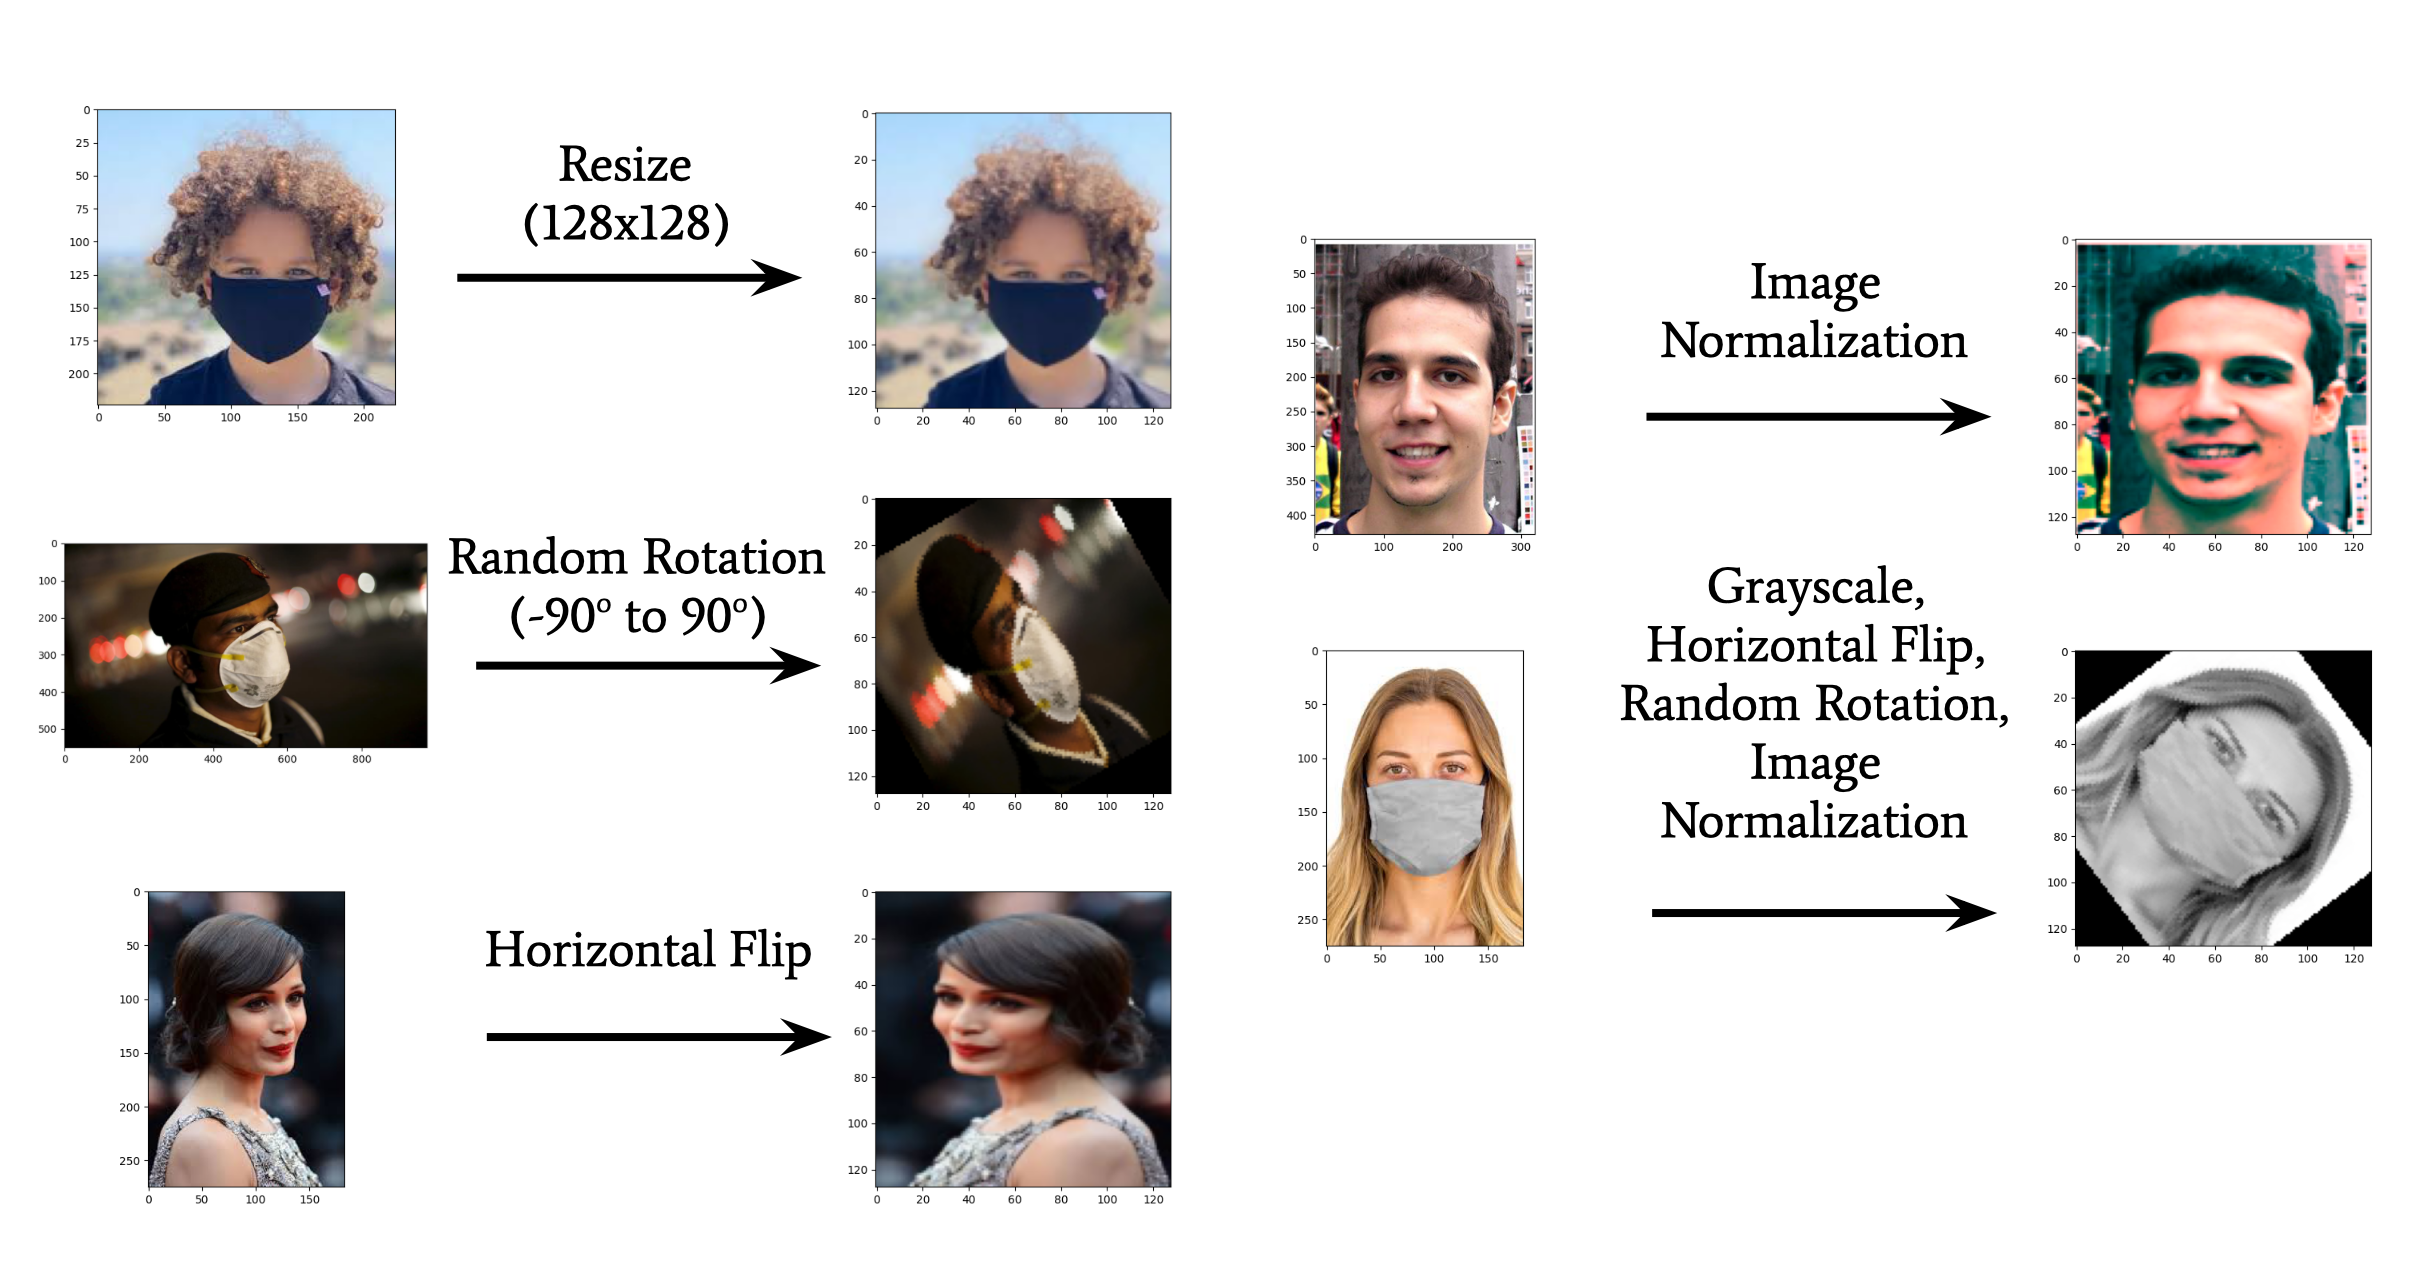
\includegraphics[height=150px]{figures/image-transformation.png}
\end{figure}